\documentclass[11pt]{article}

\usepackage[T1]{fontenc}
\usepackage[margin=0.75in]{geometry}
\usepackage{amsmath,amssymb}
\usepackage{booktabs}
\usepackage{graphicx}
\usepackage{microtype}
\usepackage{caption}
\usepackage{placeins}
\usepackage{xcolor}
\usepackage{enumitem}
\usepackage{needspace}
\usepackage{xurl}
\usepackage{hyperref}
\usepackage[backend=biber,style=numeric-comp,sorting=none,maxbibnames=3,giveninits=true,url=false]{biblatex}
\addbibresource{references.bib}
\renewcommand*{\bibfont}{\scriptsize}

\graphicspath{{figures/}}
\hypersetup{pdftitle={Longitudinal Gaps and Readout Connectivity in a Pilot Generative Model of Zero-Degree Calorimeter Showers},pdfauthor={Julian Juan},pdfsubject={Pilot calorimeter-shower model and validation-sample diagnostics},colorlinks=true,linkcolor=blue!45!black,citecolor=blue!45!black,urlcolor=blue!55!black}
\captionsetup{font=small,labelfont=bf}
\setlist{nosep,leftmargin=*}
\newcommand{\GeV}{\,\mathrm{GeV}}
\newcommand{\Kinc}{K_{\mathrm{inc}}}
\newcommand{\Y}{\mathbf{Y}}
\newcommand{\Ddev}{D_{\mathrm{dev}}}

\title{Longitudinal Gaps and Readout Connectivity in a Pilot\\Generative Model of Zero-Degree Calorimeter Showers}
\author{Julian Juan\\[3pt]\small\href{mailto:juliansjuan08@gmail.com}{juliansjuan08@gmail.com}}
\date{September 2026}

\begin{document}
\maketitle

\begin{abstract}
We examine longitudinal gaps and graph fragmentation in a hierarchical single-neutron generator for a 6,790-ID representation of an ePIC Zero-Degree Calorimeter simulation. The target is raw deposited energy, without digitization or an analysis threshold. One checkpoint trained on 26,624 showers is compared with Geant4 at 10,000 matched incident conditions spanning 50--250\,GeV kinetic energy. Among nonempty showers, the generated sample has 0.25 more active layers on average, but its last active layer lies 4.42 layers farther downstream and its occupied span contains 3.95 more inactive layers. The mean graph-component count rises from 23.42 to 59.39. Bounding the difference in occupied-layer run counts leaves an excess of at least 30.45 components within runs, or 84.6\% of the observed 35.97-component increase. Thus empty-layer separations alone do not account for the graph fragmentation. The high-level classifier AUROC of 0.775 exceeds the recorded screening maximum of 0.65. These aggregate-only results concern one training seed and a repeatedly inspected validation sample. Physical segmentation, threshold sensitivity and variation across fits remain unverified; the comparison does not establish calibrated detector performance.
\end{abstract}

\section{Introduction}

Detailed particle transport provides the reference calorimeter showers but can be computationally costly. Before detector reconstruction is considered, a surrogate can be tested against the spatial organization of its stored simulation deposits. Here, support means the set of stored channels with positive deposit; occupancy counts its members.

Generative calorimeter studies have used normalizing flows, diffusion, and conditional flow matching with regular-grid, point-cloud, or graph representations~\cite{caloflow,calodiffusion,calograph,caloclouds2,calodream}. CaloChallenge assesses complementary energy, shape, classifier, and computational-cost observables~\cite{calochallenge,kansalmetrics}. Work on the ALICE Zero-Degree Calorimeter (ZDC) has explored variational autoencoders, adversarial models, diffusion, flow matching, and mixtures of generative experts~\cite{dubinskizdc,kitazdc,fasterzdc,expertsim,wojnar2025}. Recent ZDC flow studies address output variability~\cite{majerziaf} and neighboring-channel co-activation through a Jaccard co-activation error~\cite{majerz2026}. Those models use different detector representations and targets, so their reported numerical fidelities are not direct baselines for the raw channel energies studied here.

We present a diagnostic study of a hierarchical ZDC shower generator that resolves the readout into total deposit, layer activity, and channel support. Hit-level graph networks have been used for energy and angular reconstruction in the cited ZDC design~\cite{epiczdc}, motivating tests of spatial correlations. The present graph components are diagnostics; their effect on reconstruction is not measured. We ask whether similar raw-deposit and occupancy means also imply similar longitudinal organization. Here, they coexist with deeper deposits and more inactive layers in the occupied span. We derive an aggregate bound showing that most of the component-count excess remains within occupied-layer runs. This graph diagnostic complements co-activation tests; the general need for correlation-sensitive validation is established in the cited literature.

This aggregate-only diagnostic note uses one checkpoint and 10,000 validation conditions; it tests neither architecture superiority nor detector performance.

\section{Simulation target and study population}
\label{sec:data}

\subsection{Readout target and conditioning}

The event condition is the incident-neutron four-vector $p^\mu=(E,p_x,p_y,p_z)$, expressed in GeV. The five network inputs are
\begin{equation}
 c=\left(\log(1+\Kinc/100\GeV),\,u_x,\,u_y,\,u_z,\,\log(E/\GeV)\right),
 \qquad \mathbf u=\frac{\mathbf p}{\max(\lVert\mathbf p\rVert,10^{-12}\GeV)},
 \label{eq:condition}
\end{equation}
where $\Kinc=\max(E-m_n,0)$ and $m_n=0.93956542052\GeV$. The direction features are zero at zero momentum. For $E\geq m_n$, the two energy features carry the same physical information because $E=\Kinc+m_n$. Both were used by the analyzed checkpoint; removing either changes that model. The denominator clamp is numerical.

The target $\Y\in\mathbb R_{\geq0}^{6790}$ is the raw, nondigitized energy deposited in each valid readout channel, with repeated hits to one ID summed in preprocessing. This is our data convention; Geant4 supplies the transport~\cite{geant4}. Its event total is a sum of stored readout deposits, not the incident energy or the total energy lost in detector material. No analysis threshold or additional time selection is applied; the production integration window is unknown. We call an event with zero total readout deposit an empty shower.

\subsection{Geometry and graph representation}

The stored ePIC ZDC sample has 400 electromagnetic-calorimeter (ECAL) IDs in layer 0 and 6,390 hadronic-calorimeter (HCAL) IDs in layers 1--64: 100 per layer through 63 and 90 in layer 64. Here, ``channel'' means this stored ID grouping, not a verified electronics channel. For 2,400 HCAL IDs, two to four stable positions share one ID; their unweighted centroid defines the graph node (Fig.~\ref{fig:geometry}). This observation does not establish electronic ganging. Intentional grouping and segmentation aliasing cannot be distinguished without the production ID/volume mapping. The cited design uses individually instrumented staggered tiles~\cite{epiczdc,hexplit}; its equivalence to this sample is unverified. Production geometry tag, materials, Geant4 version, physics list, cuts, field, coordinate frame and four-vector recording surface are undocumented. Layer indices are not interaction lengths; the ECAL+HCAL sum is uncalibrated.

\begin{center}
\begin{minipage}{\linewidth}
 \centering
 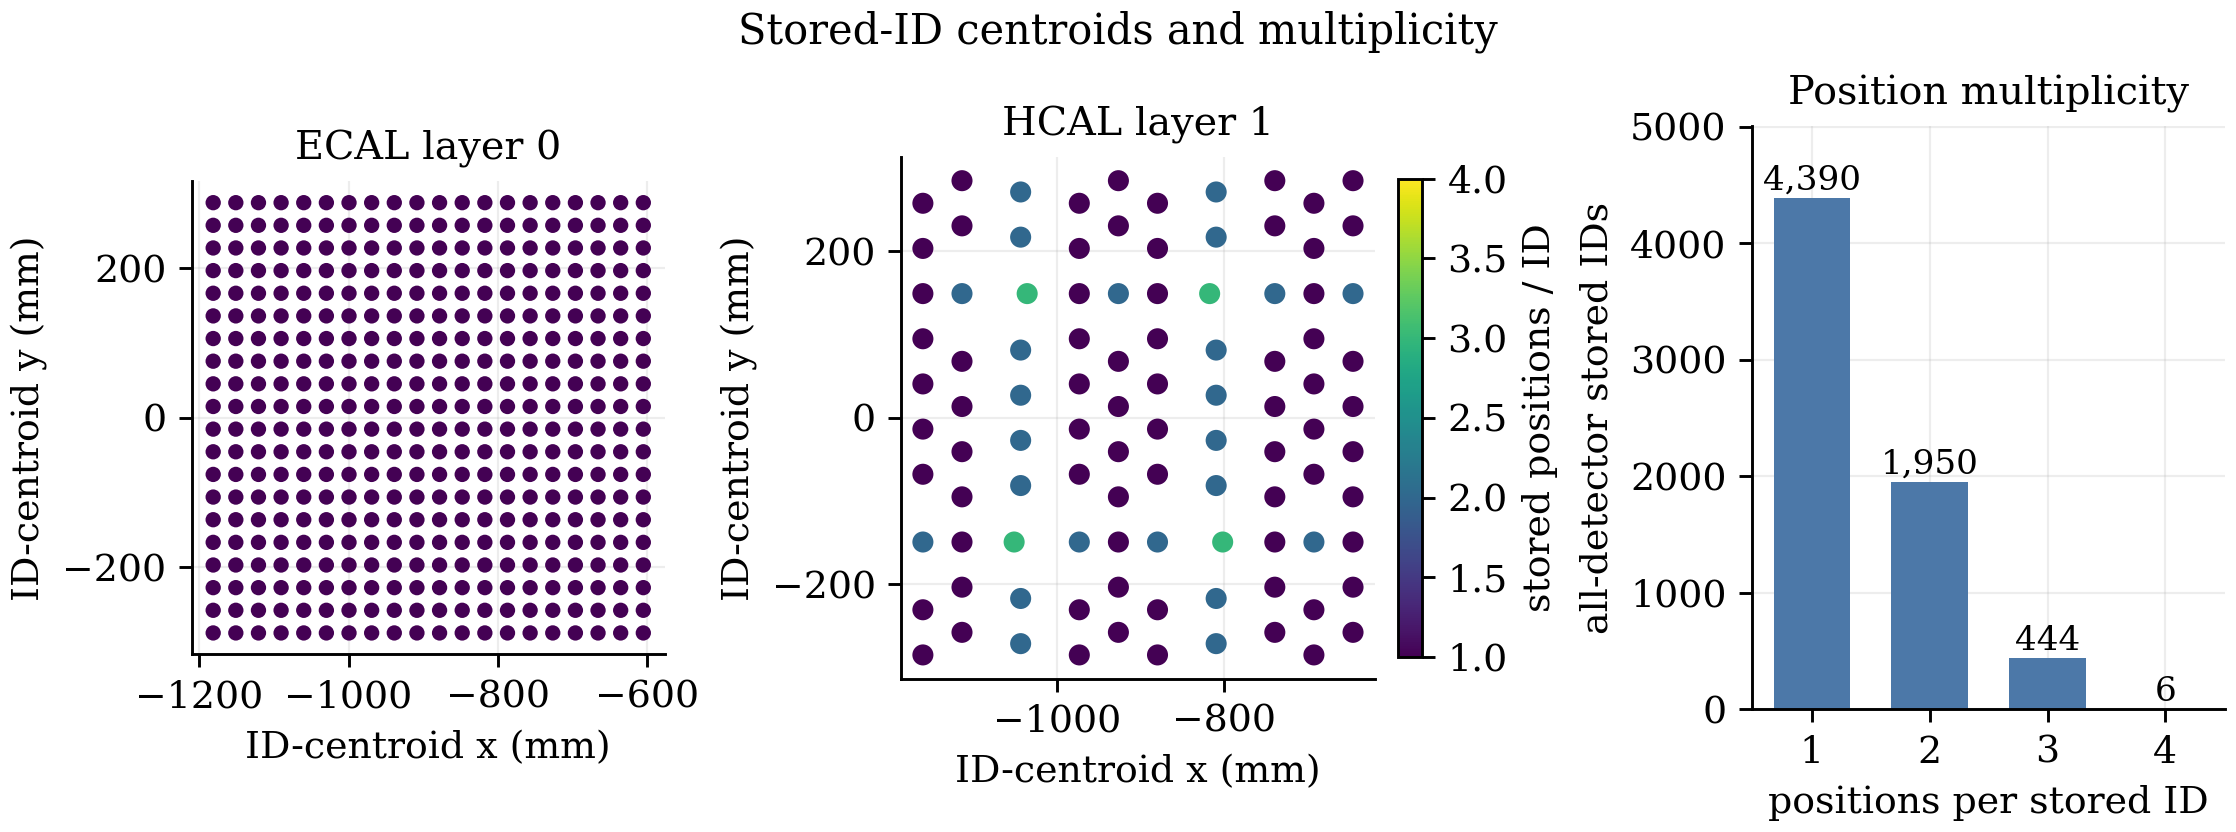
\includegraphics[width=0.94\linewidth]{detector_geometry.png}
 \captionof{figure}{Stored-ID geometry: ECAL layer 0, HCAL layer 1, and position multiplicity over all 6,790 IDs. The first bar contains 400 ECAL and 3,990 HCAL IDs. Centroids define model nodes; multiplicity does not verify physical readout ganging.}
 \label{fig:geometry}
\end{minipage}
\end{center}

The fixed graph gives each channel eight nearest-neighbor links within its layer. For each channel in layers 0--63, it also selects four nearest centroids in the next layer, with each selected longitudinal pair stored in both directions. The resulting directed edge set contains $8\times6790=54{,}320$ lateral and $2\times4\times(400+63\times100)=53{,}600$ longitudinal edges, or 107,920 in total. The generator and connectivity diagnostic share this graph, which represents adjacency through readout-centroid distances.

\subsection{Training and evaluation populations}

The preparation record contains 764,940 showers over 0--300\,GeV. A deterministic event-hash split assigns 612,482 to canonical training, 76,158 to validation, and 76,300 to the nominal test partition. The selected checkpoint instead used a pilot subset of 26,624 training and 6,656 validation events; the pilot training population is 4.35\% of canonical training.

\Needspace{8\baselineskip}
The primary shower comparison uses 10,000 incident conditions drawn from canonical validation with $50\leq\Kinc\leq250\GeV$. We refer to this repeatedly inspected validation subset as the development bank $\Ddev$. For each four-vector, we compare one stored Geant4 shower with one independently sampled model shower. The pair shares its incident condition; its stochastic shower histories are independent. The development bank's overlap with the 6,656-event pilot-validation subset cannot be reconstructed from the released aggregates, although the recorded split cross-tabulation places pilot training and validation events within their corresponding canonical partitions. No nominal test event is used here. Only aggregate reports and static geometry are available for this reanalysis; the matching event arrays and checkpoint were not recovered locally. Thus exact run counts, paired structural intervals and new generation tests cannot be reconstructed here.

\section{Generator and training procedure}
\label{sec:model}

The generator builds a shower at three levels of stored readout: event response, longitudinal allocation, and channel deposits (Fig.~\ref{fig:architecture}). It separates how much energy is stored ($T$), where along the detector it appears ($F,\mathbf A,\mathbf B$), and how it is distributed transversely ($\mathbf K,\mathbf S,\mathbf Y$). Counts precede positions, as in point-cloud models~\cite{caloclouds2,calopointflow}. These observables describe a shower outcome; the cascade does not simulate individual interactions or particle trajectories.

The model has 2,082,507 trainable parameters. A two-block residual multilayer perceptron encodes the five inputs in Eq.~\eqref{eq:condition} into a 128-component condition vector $h_c$. Discrete heads generate visibility, layer activity, channel counts, and support; two conditional flow-matching models generate the continuous layer and channel energy shares from independent Gaussian draws. There is no learned shower encoder or common random event latent. At inference, the incident four-vector is the only event input. The embedding $h_c$ encodes energy and direction for a fixed geometry; its learned coordinates have no assigned physical observables. Random draws represent conditional shower variability, not added electronics noise.

Below, $\ell=0,\ldots,64$ indexes layers, $i$ indexes valid channels in layer $\ell$, and $Y_{\ell i}$ is a stored deposit. A channel is active if $Y_{\ell i}>0$ and a layer if its budget $B_\ell=\sum_iY_{\ell i}>0$. The event total is $T=\sum_\ell B_\ell$.

\begin{center}
\begin{minipage}{\linewidth}
 \centering
 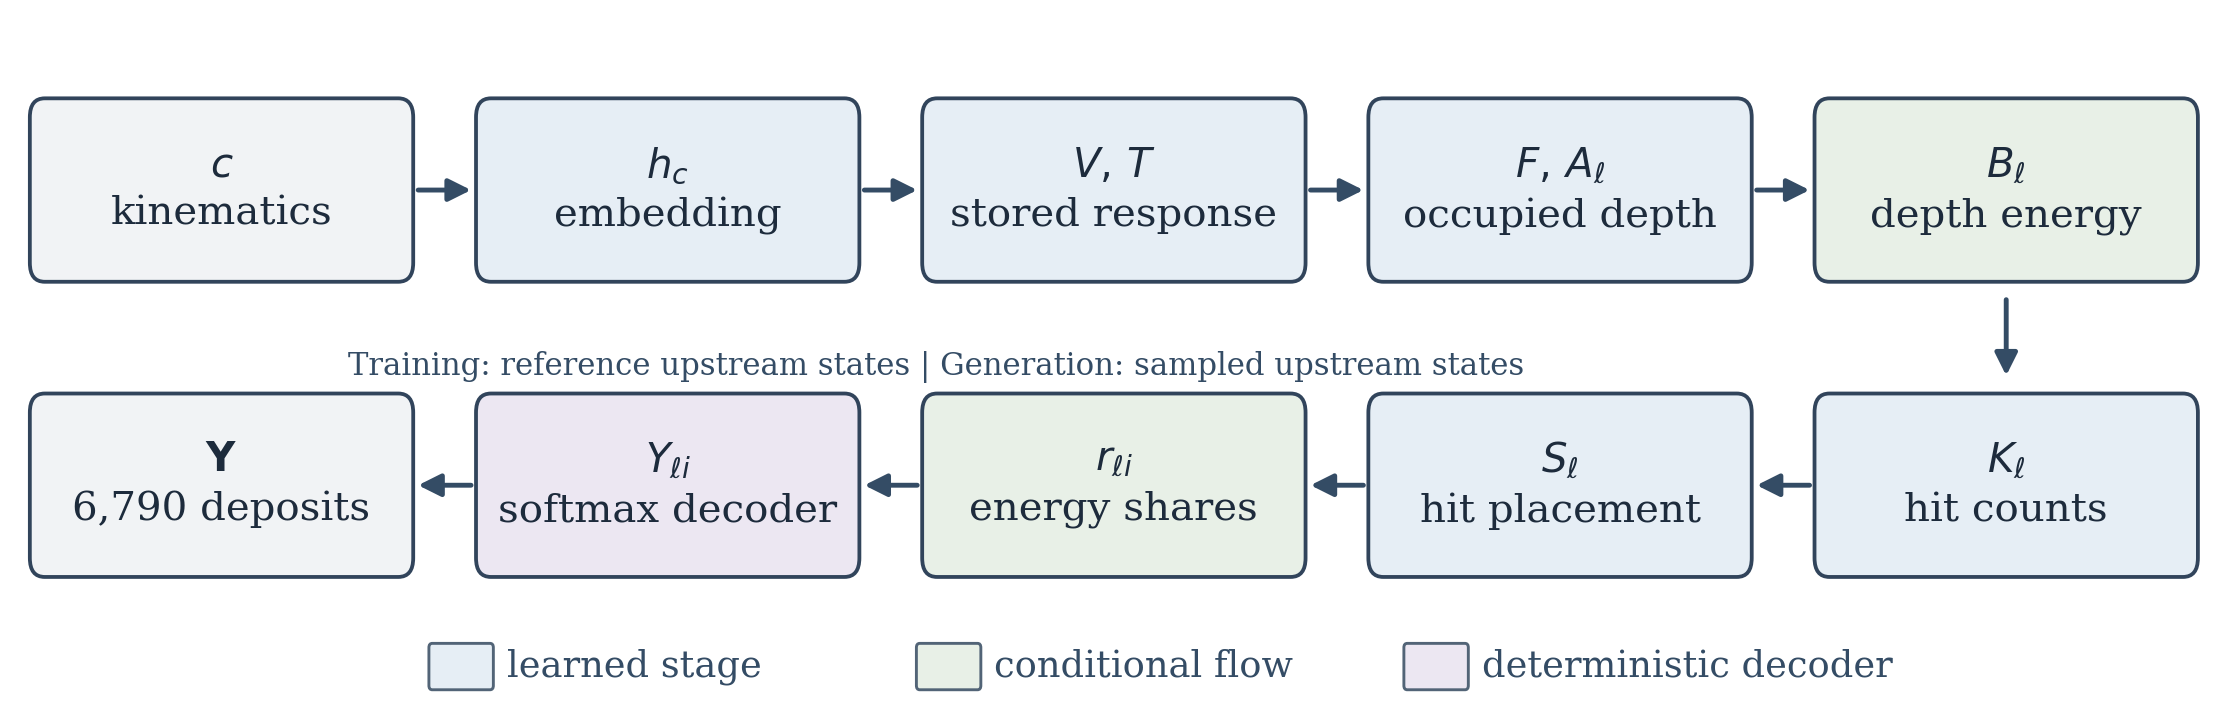
\includegraphics[width=\linewidth]{generator_schematic.png}
 \captionof{figure}{Read the top row left to right, then the bottom row right to left. The cascade maps incident kinematics to stored deposits. Green stages generate energy shares by conditional flows; purple decodes deposits. Arrows show generation order, not every conditioning connection or particle transport. The middle annotation contrasts training and generation inputs.}
 \label{fig:architecture}
\end{minipage}
\end{center}

\Needspace{8\baselineskip}
\subsection{Total deposit and longitudinal allocation}

The response stage separates zero from nonzero stored response (a hurdle model), then describes fluctuations in its magnitude. Here visibility means nonzero deposited energy, not optical visibility or the probability of an inelastic interaction. A Bernoulli head samples a provisional visibility flag $V_0$, while a four-component Gaussian mixture describes the transformed total $q_T$. The Bernoulli logit $a_\theta$, mixture means $\mu_m$, positive widths $\sigma_m$, and softmax weights $\omega_m$ depend on $h_c$; $\theta$ denotes the learned parameters and $\sigma$ the logistic function:
\begin{equation}
 \begin{aligned}
 \Pr(V_0=1\mid h_c)&=\sigma(a_\theta(h_c)),
 &q_T&=\log(1+T/10\GeV),\\
 p_\theta(q\mid h_c)&=\sum_{m=1}^{4}\omega_m(h_c)
 \mathcal N\!\left(q;\mu_m(h_c),\sigma_m^2(h_c)\right).
 \end{aligned}
 \label{eq:response_transform}
\end{equation}
A draw $q$ is mapped back to deposited-energy units, clipped at zero, and capped at the training-derived value $C(\Kinc)$. The final visibility flag also requires positive incident kinetic energy and a positive candidate deposit:
\begin{equation}
 \begin{aligned}
 C(\Kinc)&=\min\{0.630110\max(\Kinc,1\GeV),61.2338\GeV\},\\
 T_{\mathrm{cand}}&=\min\{10\GeV\max(e^q-1,0),C(\Kinc)\},\\
 V&=V_0\,\mathbf 1_{\Kinc>0}\,\mathbf 1_{T_{\mathrm{cand}}>0},
 \qquad T=VT_{\mathrm{cand}}.
 \end{aligned}
 \label{eq:cap}
\end{equation}
The cap saturates at 61.2338\,GeV above $\Kinc\approx97.2\GeV$. Its training-derived tail bound is a numerical safeguard, not a sampling fraction or a mean-response prediction. Clamping a nonpositive inverse-transform value to zero can produce an empty shower even when $V_0=1$.

For a visible event, the model draws the first active layer $F\sim\mathrm{Cat}[\operatorname{softmax}f_\theta(h_c,\log(1+T/\GeV))]$ from 65 categorical probabilities. It forces layer $F$ active and all earlier layers inactive. Separate Bernoulli draws set the later indicators $A_\ell$; conditional on $(h_c,T,F)$, their joint probability factorizes as
\begin{equation}
 p(\mathbf A\mid h_c,T,F)=\prod_{\ell>F}^{64}p(A_\ell\mid h_c,T,F,\ell),
 \qquad A_F=1.
 \label{eq:activity}
\end{equation}
$F$ marks the first stored deposit, not necessarily the first inelastic interaction. The mask $\mathbf A$ specifies occupied depth and gaps; its factorization omits residual co-activation at fixed $(h_c,T,F)$. The budget flow then assigns the longitudinal energy profile and ECAL/HCAL partition on that support. A star denotes a reference-derived quantity. For a reference shower, let $B_\ell^\star=\sum_iY_{\ell i}^\star$, $T^\star=\sum_\ell B_\ell^\star$, and $A_\ell^\star=\mathbf 1_{B_\ell^\star>0}$. The target for a nonempty event is a centered log fraction on those layers:
\begin{equation}
 a_\ell^\star=\log\max\!\left(
 \frac{B_\ell^\star}{\max(T^\star,10^{-12}\GeV)},10^{-8}\right),
 \quad (x_1)_\ell=A_\ell^\star\left(
 a_\ell^\star-\frac{\sum_m A_m^\star a_m^\star}
 {\max(1,\sum_m A_m^\star)}\right).
 \label{eq:profile_target}
\end{equation}
For an empty reference shower, the target and mask are zero. The centering removes a common log offset, leaving the relative layer shares that enter the later softmax. Floors of $10^{-8}$ and $10^{-12}\GeV$ keep the operations finite; they are numerical conventions, not detector thresholds. Floored shares are altered; their frequency is unrecorded. Centering fixes the softmax offset: targets sum to zero, whereas base noise has an extra common-offset mode. No likelihood on that singular target plane is evaluated.

Both energy-allocation flows learn a velocity field that transports Gaussian noise toward the distribution of reference log fractions, conditioned on the incident particle and upstream shower state. Flow time is an artificial interpolation coordinate, independent of detector time. Straight-path conditional flow matching regresses noise-to-target displacements~\cite{flowmatching,rectifiedflow}. For each training example, $x_0$ is standard-normal noise on the active coordinates, $x_1$ the reference-derived target, and $t$ is uniform on $[0,1]$. A mask $M_{bj}\in\{0,1\}$ identifies active coordinate $j$ of minibatch example $b$:
\begin{equation}
 x_t=(1-t)x_0+t x_1,\qquad
 \mathcal L_{\mathrm{FM}}=
 \frac{\sum_{b,j}M_{bj}
 [v_\theta(x_t,t;\mathrm{ctx})_{bj}-(x_1-x_0)_{bj}]^2}
 {\max(1,\sum_{b,j}M_{bj})}.
 \label{eq:cfm}
\end{equation}
The velocity field $v_\theta$ predicts the straight-path displacement $x_1-x_0$ from the interpolated state $x_t$, time, and context. Inactive coordinates do not contribute to the masked squared-error loss.

\Needspace{8\baselineskip}
During generation, both flows start from fresh Gaussian noise and use eight masked velocity updates. The context contains outputs sampled by earlier stages, whereas training supplies their reference values. For an active-layer or selected-channel mask $M$, the implemented rule is
\begin{equation}
 z_0=M\odot\varepsilon,\quad \varepsilon\sim\mathcal N(0,I),\qquad
 z_{n+1}=M\odot\left[z_n+\tfrac18
 v_\theta\!\left(z_n,\tfrac{n+1/2}{8};\mathrm{ctx}\right)\right],
 \quad n=0,\ldots,7.
 \label{eq:flow_steps}
\end{equation}
Here $\odot$ denotes elementwise multiplication. Each update evaluates the velocity at the current state $z_n$ and the midpoint \emph{time} $(n+1/2)/8$, then resets inactive coordinates to zero. It is a first-order explicit update with midpoint-time evaluation, not the midpoint Runge--Kutta method, which also advances the state to the midpoint. For a visible event, the resulting active-layer logits are normalized to fractions $\pi_\ell$, giving budgets
\begin{equation}
 \pi_\ell=\frac{A_\ell e^{z_{8,\ell}}}
 {\sum_{m:A_m=1}e^{z_{8,m}}},\qquad
 B_\ell=T\pi_\ell,\qquad \sum_{\ell=0}^{64}B_\ell=T.
 \label{eq:layer_budget}
\end{equation}
Only active layers enter the softmax denominator; their budgets sum to the sampled total and inactive layers receive zero. The layer-flow network uses a 128-component representation and two bidirectional transformer layers with four attention heads. Its context includes $h_c$, the total $T$, layer identity, the activity mask, and a sinusoidal flow-time encoding. Bidirectional attention lets each layer use information from all other layers; it is a statistical dependency, not backward particle transport.

\subsection{Channel count, support, and deposited energy}

Given $(h_c,B_\ell,A_\ell)$ and a learned layer identifier, a categorical head draws the number $K_\ell$ of active channels. A feasibility mask sets $K_\ell=0$ for inactive layers and restricts active layers to $1\leq K_\ell\leq N_\ell$, where $N_\ell$ is the number of valid channels. This models readout multiplicity at a given layer energy. It does not specify particle multiplicity, footprint area, channel positions or a minimum deposit.

The support network uses channel geometry and the sampled layer state to score candidate channels. Its inputs combine standardized $(x,y,z)$ centroids, normalized layer index, ECAL/HCAL indicators, $h_c$, $B_\ell$, and the requested fraction $K_\ell/N_\ell$. Three graph blocks of width 96 propagate information along the fixed directed edge set $\mathcal E$. Each block forms messages from neighboring readouts and uses their sum to update the receiving channel. If $h_i^{(r)}$ is the representation of channel $i$ entering block $r$, and $e_{ji}$ contains five edge inputs (three coordinate differences, distance, and edge type), one block computes
\begin{equation}
 m_i^{(r)}=\sum_{j:(j,i)\in\mathcal E}
 \phi_r(h_j^{(r)},h_i^{(r)},e_{ji}),\qquad
 h_i^{(r+1)}=h_i^{(r)}+\psi_r(h_i^{(r)},m_i^{(r)}).
 \label{eq:message}
\end{equation}
Here $\phi_r$ computes each message and $\psi_r$ computes the residual update. Layerwise averages of the resulting representations pass through a two-layer, four-head bidirectional transformer; its outputs are broadcast back to channels before their final scores $s_{\ell i}$ are formed. Messages let scores depend on nearby readouts; they are statistical comparisons, not particle or energy transport. The support $S_\ell$ determines transverse placement and therefore graph connectivity. Selection is a separate stochastic step. For valid-channel set $\mathcal N_\ell$, the sampler chooses
\begin{equation}
 S_\ell=\left\{i\in\mathcal N_\ell:
 \operatorname{rank}_{\mathcal N_\ell}(s_{\ell i}/\tau+g_{\ell i})\leq K_\ell\right\},
 \label{eq:topk}
\end{equation}
Rank one denotes the largest noisy score. The sampler uses temperature $\tau=1$ and independent Gumbel perturbations $g_{\ell i}$ obtained from uniform draws clipped to $[10^{-7},1-10^{-7}]$~\cite{gumbeltopk}. Gumbel-top-$K$ samples $K_\ell$ distinct channels without replacement. Selecting the top $K_\ell$ enforces the requested count exactly, but imposes no adjacency or connectivity constraint.

\Needspace{12\baselineskip}
A second flow divides each layer budget among its selected channels, describing energy concentration and fluctuations on fixed support. It can change energy-weighted shape and centroids, but cannot relocate deposits or repair disconnected support in exact arithmetic. In training, $S_\ell^\star$ denotes the positive-deposit reference channels and $K_\ell^\star=|S_\ell^\star|$. For $K_\ell^\star>0$, its target is the centered log fraction of each channel's layer budget:
\begin{equation}
 a_{\ell i}^\star=\log\max\!\left(
 \frac{Y_{\ell i}^\star}{\max(B_\ell^\star,10^{-12}\GeV)},10^{-8}\right),\qquad
 (x_1)_{\ell i}=\mathbf 1_{i\in S_\ell^\star}
 \left(a_{\ell i}^\star-\frac{1}{K_\ell^\star}
 \sum_{j\in S_\ell^\star}a_{\ell j}^\star\right).
 \label{eq:share_target}
\end{equation}
Here $x_1$ refers to the channel-flow target rather than the layer-flow target. The centering preserves the floored relative shares. An inactive layer has zero target coordinates. This flow uses Eqs.~\eqref{eq:cfm} and \eqref{eq:flow_steps} with the reference channel set during training and the sampled set during generation.

The channel-flow velocity network follows the support network's graph and layer-context design, with the flow state and a sinusoidal time encoding supplied at each channel. Unselected channels are masked before and after every graph block. Eight updates yield logits $r_{\ell i}$ for selected channels; a deterministic softmax then assigns the energy
\begin{equation}
 Y_{\ell i}=
 \begin{cases}
 B_\ell\,\dfrac{\exp r_{\ell i}}{\sum_{j\in S_\ell}\exp r_{\ell j}}, & i\in S_\ell,\\[6pt]
 0, & i\notin S_\ell,
 \end{cases}
 \label{eq:decoder}
\end{equation}
Consequently, in exact arithmetic, $|S_\ell|=K_\ell$, $Y_{\ell i}\geq0$, $\sum_iY_{\ell i}=B_\ell$, and $\sum_{\ell i}Y_{\ell i}=T$. These are accounting identities for the model's sampled readout budget, not conservation of the incident neutron's full energy. Energy in unrecorded material and leakage are not generated; positivity and closure alone do not establish a physical shower.

\subsection{Training and checkpoint selection}

Each training component receives reference-derived targets and upstream values (teacher forcing). During generation, it receives their sampled values, allowing errors to propagate through the cascade. We therefore evaluate complete generated showers (free-running generation) in Sec.~\ref{sec:results}. The joint training objective combines nine weighted losses:
\begin{equation}
 \begin{aligned}
 \mathcal L_{\rm joint}={}&w_V\mathcal L_{\rm BCE}(V)
 +w_T\mathcal L_{\rm NLL}(T)
 +w_F\mathcal L_{\rm CE}(F)
 +w_A\mathcal L_{\rm BCE}(\mathbf A)
 +w_B\mathcal L_{\rm FM}^{B}\\
 &+w_K\mathcal L_{\rm CE}(\mathbf K)
 +w_S\mathcal L_{\rm BCE}(\mathbf S)
 +w_R\mathcal L_{\rm rank}(\mathbf S)
 +w_Y\mathcal L_{\rm FM}^{Y}.
 \end{aligned}
 \label{eq:joint_loss}
\end{equation}
Binary cross entropy (BCE) trains visibility, later-layer activity, and channel-support decisions; categorical cross entropy (CE) trains first-layer and count distributions. The total-deposit negative log likelihood (NLL) uses the density in transformed $q_T$. Expressing that density in deposited-energy units introduces the Jacobian factor $1/(T+10\GeV)$. The ranking term averages $\log[1+\exp(-(s_i-s_j))]$ over sampled occupied--unoccupied channel pairs. Superscripts $B$ and $Y$ denote the masked layer-budget and channel-share flow losses in Eq.~\eqref{eq:cfm}; the count loss downweights zeros in inactive layers.

The retained calibration proposal uses training-data gradient norms to set $w_j$. In that proposal, response, layer-profile, and count weights hit the lower clipping bound; the visibility weight hit the upper bound. The bounds apply before normalization of the weights to mean one. Appendix~\ref{app:reproducibility} records the calibration values and their provenance limits. A weight-sensitivity study would test whether these bounds affect shower structure.

Optimization proceeded through response, profile, count, support, share, and joint stages. The condition encoder was trained with the response head, frozen for the intermediate component stages, and unfrozen for joint training. Each stage inherited the preceding checkpoint; freezing the encoder kept the inputs to previously trained heads fixed during intermediate stages.

Training used AdamW with a peak learning rate of $3\times10^{-4}$, batches of six accumulated over four steps (effective batch size 24), gradient clipping at one, and seed 20260723. Epoch 90 minimizes the teacher-forced validation objective across 104 retained rows spanning epochs 11--114 and defines the checkpoint analyzed below. Selection used this objective; the free-running support diagnostics were evaluated subsequently. The checkpoint need not minimize those free-running discrepancies.

\section{Evaluation protocol}
\label{sec:diagnostics}

We examine the generated readout at three scales: total and section deposits, longitudinal layer structure, and channel-level support. Response measurements include empty showers and are summarized both over the full sample and in eight 25\,GeV incident-energy bins. Numerical checks test the generated deposits against the model's sampled budgets, while distributional comparisons assess agreement with Geant4.

\Needspace{9\baselineskip}
Support measurements use a strictly positive energy definition; no detector or analysis threshold is applied. For a nonempty shower, let $F$ and $L$ be the first and last active layers, and $A_\ell$ the activity indicator. The occupied span is $L-F+1$ and the number of inactive layers within it is
\begin{equation}
 G=L-F+1-\sum_{\ell=0}^{64}A_\ell.
 \label{eq:gaps}
\end{equation}
This counts inactive layers, not contiguous runs. An interior gap occurs when $G>0$. We also count active channels and weakly connected components $C_1,\ldots,C_m$ of their induced subgraph, ignoring edge direction, and report the largest-component fraction $\max_j|C_j|/|S|$ for occupied set $S$. A component is a group of occupied channels joined by paths using only occupied channels. These support metrics condition on nonempty readout, leaving 9,907 reference and 9,858 generated showers. The two nonempty subsets need not contain the same incident conditions.

The component count depends on longitudinal activity even if within-layer support were unchanged. Graph edges join only the same or adjacent layers. If $R$ is the number of maximal runs of occupied layers, then $m\geq R$: an empty layer between two occupied runs blocks every path between them. Consecutive empty layers constitute one separation, so $G$ alone specifies neither $R$ nor lateral fragmentation. For example, occupied layers $1,2,5$ have span five, $G=2$, and $R=2$, whereas $1,3,5$ has the same span and $G$ but $R=3$. Define $Q=m-R$, the component count beyond one per occupied-layer run. Writing $I=\mathbf 1_{G>0}$ gives $1+I\leq R\leq G+1$: any interior gap requires at least two occupied runs. Thus $\overline m-1-\overline G\leq\overline Q\leq\overline m-1-f$, where $f=\overline I$ is the nonempty gap fraction. Subtracting the separate sample bounds gives
\[
 \Delta\overline m-\overline G_{\rm gen}+f_{\rm ref}\leq\Delta\overline Q
 \leq\Delta\overline m+\overline G_{\rm ref}-f_{\rm gen},
 \qquad \Delta=\mathrm{generator}-\mathrm{reference}.
\]
This deterministic aggregate bound is not a confidence interval or causal decomposition. With event activity masks, $R$ and $Q$ could be computed exactly; the aggregate report does not retain them. Components characterize graph-defined support, not detector-reconstruction clusters~\cite{atlastopocluster}.

For all-event active-channel counts, including empties, the one-dimensional Wasserstein distance $W_1$ is the area between empirical cumulative distributions, in channels~\cite{kansalmetrics}. The 95\% percentile intervals for $W_1$ and the zero-deposit fraction difference use 1,000 bootstrap resamples, stratified by incident-energy bin and preserving matched pairs. Intervals for the energy-bin differences, mean longitudinal profile, gaps, and graph components are unavailable. All quoted intervals describe resampling variation within the development bank.

A classifier two-sample test (C2ST) distinguishes generated from reference showers; AUROC (area under the receiver operating characteristic curve) has chance benchmark 0.5~\cite{c2st,kansalmetrics}. The original three-seed battery uses a row-wise split. Members of a matched condition pair can enter opposite partitions; its condition-only AUROC of 0.464 is a failed control consistent with opposite-label twin bias. A separate pair-grouped monitor records the same run and epoch (\texttt{dicos-f-02}, epoch 90), with condition-only/high-level AUROCs 0.500/0.893. Its different event sample precludes a direct comparison. Appendix~\ref{app:additional} gives the seeds and recovered evaluator specification.

\Needspace{12\baselineskip}
\section{Results}
\label{sec:results}

Table~\ref{tab:results} compares deposits over all 10,000 conditions and support over separately nonempty samples. Similar mean deposit and activity coexist with larger longitudinal spans, gap counts and graph-component counts.

\begin{center}
\begin{minipage}{\linewidth}
\centering
\captionof{table}{Aggregate comparison on the development bank. Deposit means and zero-deposit counts use all 10,000 matched conditions; support means use nonempty showers (9,907 Geant4 and 9,858 generated). Differences are generator minus reference, computed before rounding; pp denotes percentage points.}
\label{tab:results}
\small
\begin{tabular}{@{}lrrr@{}}
\toprule
Quantity & Geant4 reference & Generator & Gen. $-$ ref. \\
\midrule
Zero-deposit events & 93 (0.93\%) & 142 (1.42\%) & $+49$ ($+0.49$ pp) \\
Mean total deposit (GeV) & 4.324 & 4.369 & $+0.045$ \\
Mean ECAL deposit (GeV) & 2.100 & 2.275 & $+0.175$ \\
Mean HCAL deposit (GeV) & 2.224 & 2.094 & $-0.129$ \\
\midrule
Mean first active layer & 0.510 & 0.735 & $+0.225$ \\
Mean last active layer & 56.20 & 60.62 & $+4.42$ \\
Mean active layers & 54.58 & 54.83 & $+0.25$ \\
Mean occupied span & 56.69 & 60.88 & $+4.20$ \\
Mean inactive layers in span & 2.10 & 6.05 & $+3.95$ \\
Events with an interior gap & 52.43\% & 93.53\% & $+41.10$ pp \\
Mean active channels & 1617.6 & 1588.8 & $-28.7$ \\
Mean weak graph components & 23.42 & 59.39 & $+35.97$ \\
Mean largest-component fraction & 94.90\% & 88.87\% & $-6.03$ pp \\
\bottomrule
\end{tabular}
\end{minipage}
\end{center}

\subsection{Deposited energy and empty showers}

The all-event mean total deposit is 4.369\,GeV for generated showers and 4.324\,GeV for Geant4, a difference of 0.045\,GeV (1.0\%). The similar total means conceal opposing section-level shifts: generated ECAL deposit is higher by 0.175\,GeV (8.3\%) and HCAL deposit lower by 0.129\,GeV (5.8\%) (Table~\ref{tab:results}). Figure~\ref{fig:longitudinal} shows their mean longitudinal allocation. At the reference HCAL maximum (layer 9), the generated mean is 8.6\% lower. Mean profiles cannot reveal individual interior gaps.

\begin{figure}[!htbp]
 \centering
 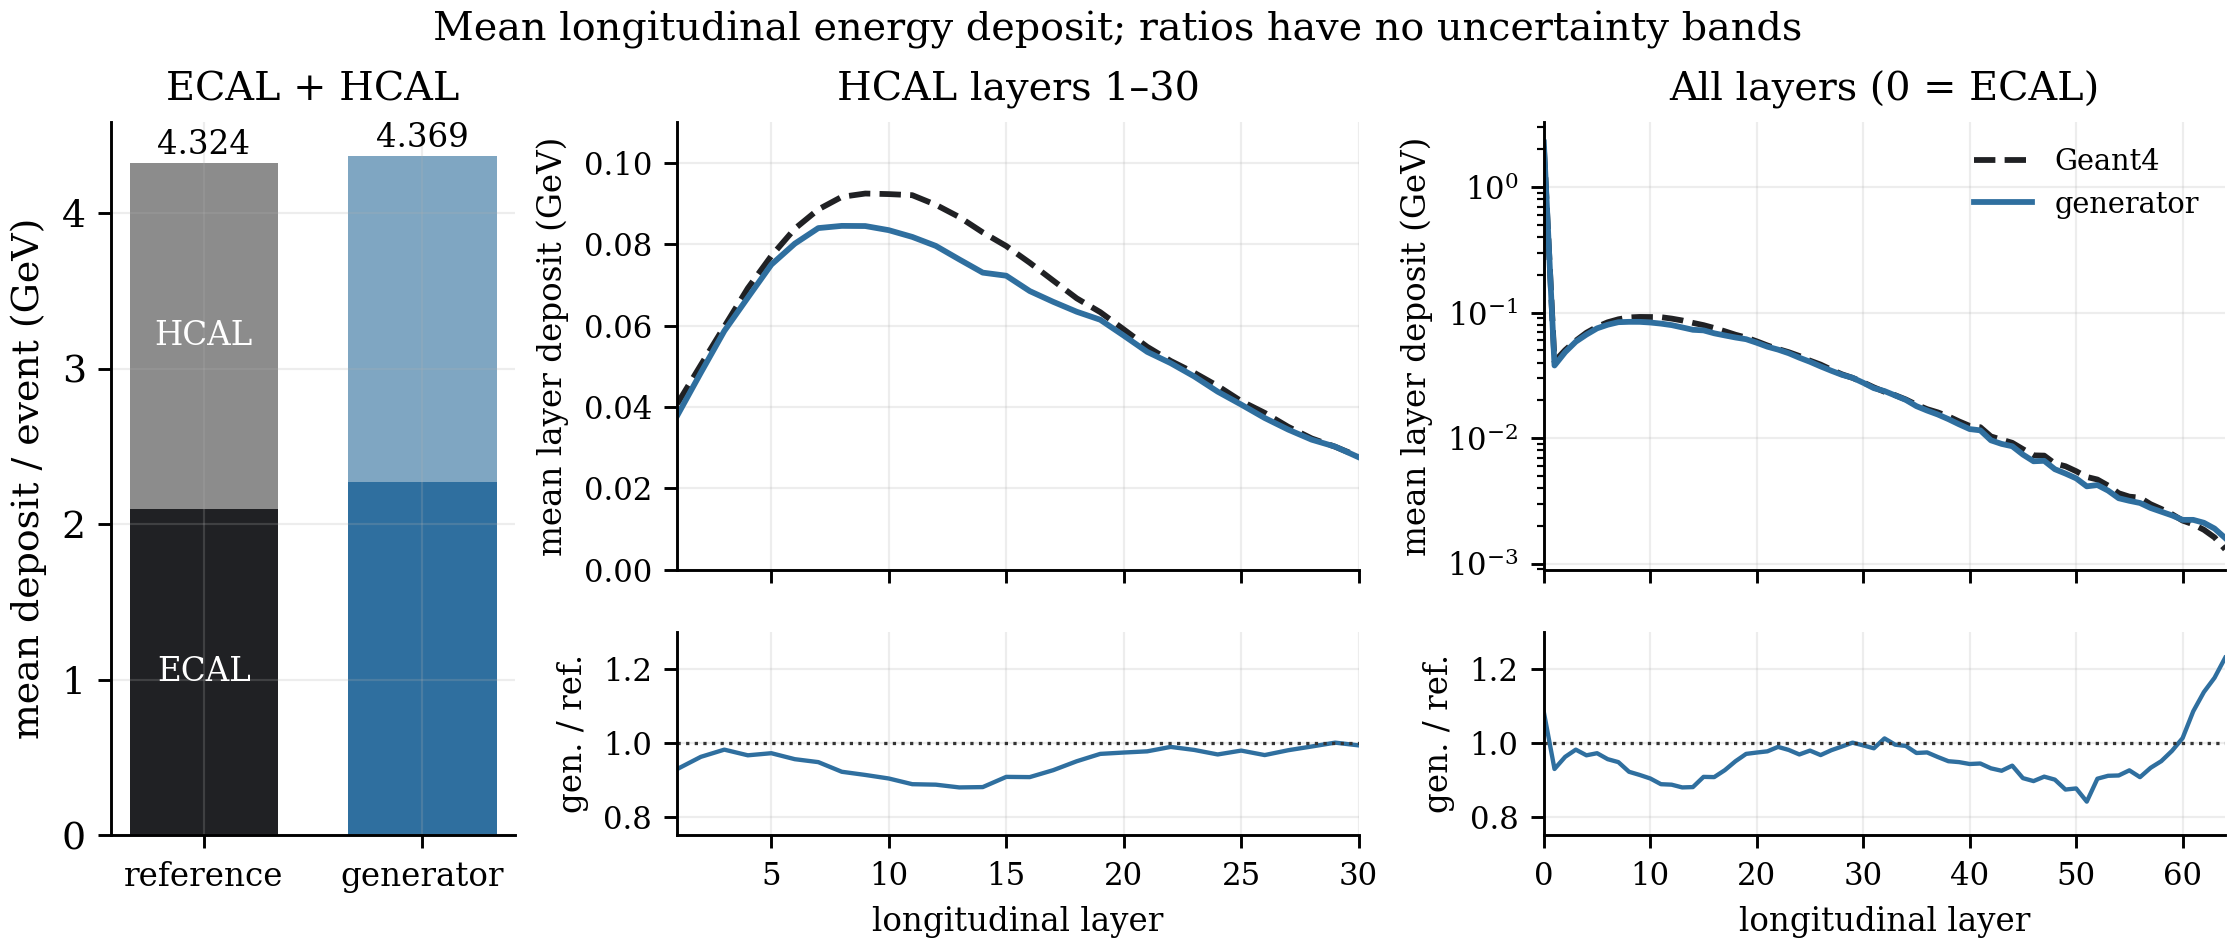
\includegraphics[width=\linewidth]{longitudinal_profile.png}
 \caption{Mean deposited energy over all 10,000 development-bank events. Left: ECAL and HCAL deposits expose section-level compensation. Center: HCAL layers 1--30 (linear scale). Right: all layers, including ECAL at 0 (log scale). Dashed curves denote Geant4, solid curves the generator. Lower panels show ratios of means; uncertainty bands are unavailable. Empty showers are included.}
 \label{fig:longitudinal}
\end{figure}

Table~\ref{tab:energy_bins} gives binwise means, standard deviations and relative differences. Pooling the bin moments gives all-event standard deviations of 4.759 and 4.830\,GeV for reference and generator. The paired covariance is unavailable, so neither significance of the 0.045\,GeV mean difference nor a sampling-noise explanation of the binwise fluctuations is established.

The model produces 142 empty showers versus 93 in Geant4, a difference of 49 events or 0.49 percentage points. The paired-bootstrap 95\% percentile interval for this fraction difference is 0.19--0.76 percentage points. The corresponding nonempty samples contain 9,858 generated and 9,907 reference showers. The report's visibility labels do not retain provisional $V_0$, so the 142 generated zeros cannot be split reliably into hurdle and clamp contributions.

\subsection{Longitudinal activity}

The generated showers have nearly the same mean number of active layers as the reference (54.83 versus 54.58), but the occupied layers lie farther downstream. Their mean first active layer shifts by $+0.225$ and last active layer by $+4.42$. The nonempty fraction starting in ECAL is 92.53\% versus 93.81\%. The occupied span grows by $+4.20$ layers while the count of active layers grows by only $+0.25$, leaving $+3.95$ inactive layers inside the span. The fraction of nonempty showers with an interior gap rises from 52.43\% to 93.53\% (Table~\ref{tab:results}). For nonempty showers, mean energy-weighted depth, $\sum_\ell\ell B_\ell/\max(T,10^{-9}\GeV)$, is instead 14.14 for the generator and 14.15 for Geant4. Including empty events as zeros gives 13.94 and 14.02, respectively. This distinguishes occupied extent from energy-weighted depth, but does not determine the energy carried by disconnected components. Figure~\ref{fig:support} bounds the within-run fragmentation.

\begin{figure}[!htbp]
 \centering
 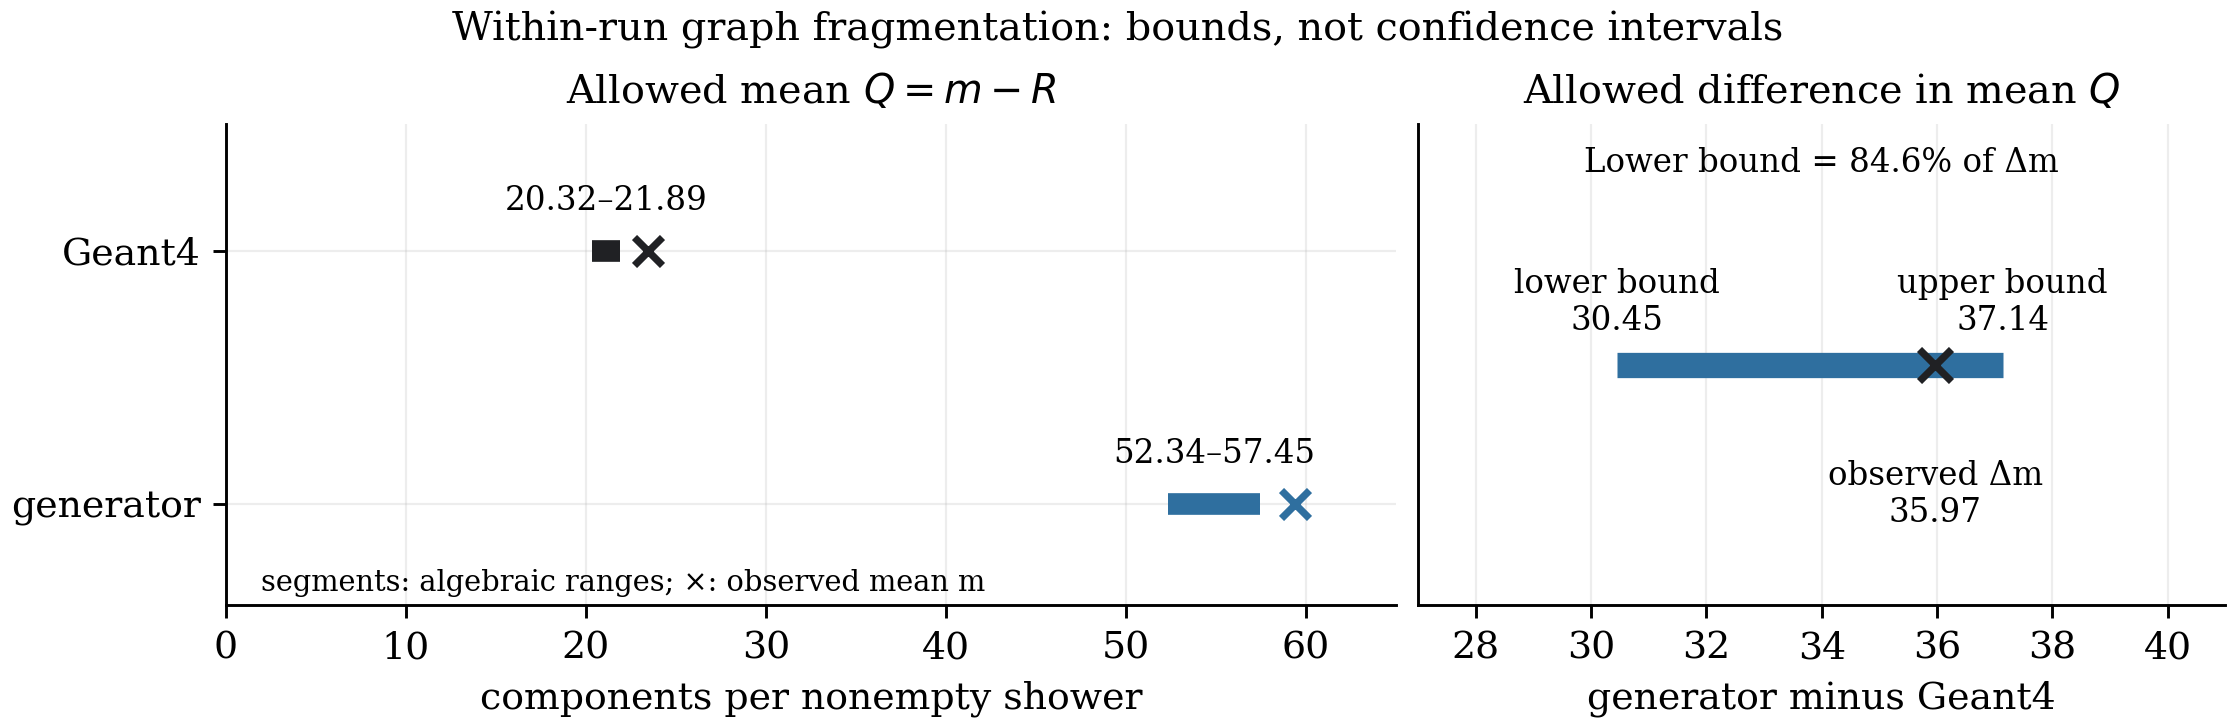
\includegraphics[width=\linewidth]{support_summary.png}
 \caption{Graph fragmentation conditional on nonempty readout (9,907 Geant4 and 9,858 generated showers). Left: observed mean component counts $m$ (crosses) and allowed ranges of $Q=m-R$ (segments). Right: the allowed difference in mean $Q$ compared with the observed difference in mean $m$. Ranges use $1+\mathbf 1_{G>0}\leq R\leq G+1$; they are algebraic bounds, not uncertainty intervals. All quantities use strictly positive deposits and the model graph.}
 \label{fig:support}
\end{figure}

\subsection{Channel support and graph structure}

Generated showers have 28.7 fewer active channels on average, but 35.97 more weak components on the model graph. The largest component contains 88.87\% of occupied channels on average, versus 94.90\% in the reference. The all-event active-channel-count distribution has $W_1=58.68$ channels, with a paired-bootstrap 95\% interval of 51.47--66.92 channels. This distance includes the zero-count mass, whereas the means above condition on nonempty showers. Two retained reference-half splits give 13.78 and 15.82 channels (5,000 events per half). These are finite-sample comparison scales, not critical values or matched-size significance estimates.

The fraction of directed graph edges whose endpoints are both occupied averages 0.1375 for the generator and 0.1458 for Geant4 over all 10,000 events. This measures local co-occupancy on the same graph, but is not normalized for occupancy and does not isolate a correlation discrepancy.

\subsection{Classifier and numerical checks}

The original C2ST battery gives mean AUROCs of 0.775 for high-level shower summaries, 0.791 for channel energies and 0.856 for layer profiles across three classifier seeds. Its high-level score exceeds the recorded screening maximum of 0.65. The failed condition-only control prevents a calibrated fidelity interpretation; a pair-grouped rerun on the same bank is needed. These scores and the failed criterion remain as provenance, not percentages of physically incorrect showers.

The evaluator uses a common event/layer residual tolerance: the larger of $2\times10^{-5}$\,GeV and $10^{-5}$ times the largest sampled event total in each batch. All 1,250 batches of eight passed, with no nonfinite/negative deposit or invalid support/count/mask. The zero support-mask mismatch verifies that FP32 decoding created no selected-but-empty channels in this sample; such losses would bias support metrics. Maximum event and layer residuals were $1.14\times10^{-5}$ and $3.05\times10^{-5}$\,GeV. The maximum layer residual exceeds the earlier fixed $2\times10^{-5}$\,GeV criterion; the reported pass applies specifically to the batch-dependent criterion.

\FloatBarrier
\section{Discussion}
\label{sec:discussion}

\subsection{Interpretation and diagnostic tests}

Graph connectivity distinguishes more than empty-layer separations. The bound in Sec.~\ref{sec:diagnostics} gives $\overline Q_{\rm gen}\geq52.34$ and $\overline Q_{\rm ref}\leq21.89$, hence $\Delta\overline Q\geq30.45$: at least 84.6\% of the observed 35.97-component excess remains beyond one component per occupied run. This establishes a within-run graph-fragmentation discrepancy in these samples. It does not identify a purely lateral effect: adjacent occupied layers may also fail to connect through the selected edges. Nor does it assign a causal percentage to a model stage. The separately nonempty populations need not share the same incident conditions.

Equation~\eqref{eq:activity} assumes conditional independence of later-layer activity given $(h_c,T,F)$. In a three-layer example, fix $F=0$ and let layers 1 and 2 be jointly active with probability $p$. Independent draws with the same marginals preserve the mean active-layer count but give an interior-gap probability $p(1-p)$ instead of zero and increase the mean last layer by $p(1-p)$. This explains a possible signature, not the measured magnitude. Sampled $T$ and $F$ can still induce dependence when their values vary; the first deposited layer is not necessarily the first inelastic-interaction depth.

A reference activity null controlling energy, direction, $T$ and $F$ would test whether factorization reproduces the depth and gap shifts. An oracle cascade must replace the full activity mask; reference $T$ and $F$ alone leave the factorization intact. L2LFlows and iCaloFlow model interlayer dependence~\cite{l2lflows,icaloflow} and motivate a matched comparison.

BCE-trained logits are not automatically calibrated inclusion probabilities after fixed-count Gumbel selection. Independent channel perturbations can disrupt connected support even with smooth scores. Occupancy calibration conditional on layer and count, and a matched-marginal placement null, would test that hypothesis. The channel flow cannot repair selected support in exact arithmetic. Shared random upstream states and cross-layer attention can nevertheless induce centroid correlations without a common event latent; measuring those correlations would test shower-axis coherence.

\subsection{Limitations and robustness}

Paired sampling intervals for the headline structural means are not retained. Large descriptive differences do not establish robustness across training seeds, thresholds or graphs. A three-seed study and full-data fit are needed to separate architecture effects from training-population and optimization effects.

Strict-positive support is a property of stored simulation deposits, not electronics readout. Soft or late deposits can change gaps and components; their contribution cannot be quantified without channel-energy spectra and time information. Detector-specific threshold and integration-window studies, and an independently defined physical-neighbor graph, are needed before interpreting the graph discrepancy as detector performance. The cited design uses a 0.5\,MeV MIP scale, a reconstructed-hit cut above 0.5 MIP and $t<275$\,ns~\cite{epiczdc}. These motivate a 0.25\,MeV HCAL sensitivity scan, but transferring the cuts requires the production segmentation and timing convention; a reference-only time cut would compare different targets.

The incident four-vector omits an explicit impact position. Whether direction determines that position depends on the production vertex and recording surface, which need verification. Position-conditioned residuals and the joint empty-shower contingency table would test whether conditioning and geometric acceptance are learned; marginal empty fractions alone cannot answer this.

Training loss averages updating minibatches, whereas validation uses the epoch-end model in the available implementation; historical runtime identity is unverified. Response-tail studies require counts of generated draws clipped by the cap and reference deposits above it. Numerical sensitivity requires a solver-step study. A locked bank with verified identities and repeated generation at fixed conditions is also needed.

\subsection{Computational performance and detector applications}

The evaluator timing includes topology and classifier tests; generation latency was not isolated. A matched end-to-end benchmark must include both solvers, decoding and output handling, with hardware and batch size specified for generator and Geant4.

Relating this raw-deposit study to detector performance requires production metadata, training-only calibration applied unchanged to both samples, and energy and position reconstruction. The ECAL and HCAL shifts cancel only in the unweighted stored-energy sum. A sampling fraction from another production cannot establish this model's calibrated bias.

\Needspace{10\baselineskip}
\section{Conclusion}

This pilot comparison shows that similar mean energy and occupancy do not imply matched longitudinal or graph structure. A difference of 0.25 active layers coexists with a last active layer shifted by 4.42 layers and 3.95 additional inactive layers in the occupied span. At least 30.45 of the 35.97 excess components remain within occupied-layer runs. Empty-layer separations are therefore insufficient to explain fragmentation on this graph. Connecting this descriptive result to detector performance requires conditional activity and support-sampling tests, threshold and graph sensitivity, and reconstruction studies.

\section*{Code and data availability}

The \href{https://github.com/JulianAttemptsCoding/fast-mc-paper}{project repository} provides aggregate reports, geometry, training history, figure scripts and manuscript source; its README identifies revisions and build audits. The collaboration-owned events and checkpoint are not redistributed. Generation, retraining and event-level studies require those resources.

\section*{Acknowledgments}

The author thanks Dr. Wen-Chen Chang (Institute of Physics, Academia Sinica) for his generous mentorship, guidance, and encouragement, and the Institute of Physics laboratory community for their welcome and support.

\section*{Author contributions and use of generative AI}

Julian Juan: conceptualization, methodology, software, investigation, visualization, and writing.

OpenAI Codex assisted with software and manuscript drafting, specification review, literature searches, and editing. The author supplied the research ideas, checked the work, and takes responsibility for the scientific content.


\Needspace{10\baselineskip}
\appendix
\section{Recorded settings and reproducibility limits}
\label{app:reproducibility}

The analyzed checkpoint is \texttt{dicos-f-02}, epoch 90, from the \texttt{calibrated\_lr3e4} family, with training seed 20260723. Its SHA-256 is
\begin{quote}\footnotesize\nolinkurl{491284c7423f365230d34b0443f95aa4888ec770bdc673c4c979897bad8acbce}\end{quote}
and its recorded frozen-configuration SHA-256 is
\begin{quote}\footnotesize\nolinkurl{116bc8c220b07ce54ae07196bdd6ed8e835775c8c937182a209a799dc94ae9c5}\end{quote}
The selected validation objective is 4.4837676194. The recorded lineage includes a declared learning-rate restart between epochs 70 and 71, followed by annealing; it is not one uninterrupted decay. The retained history covers epochs 11--114. The original runtime configuration, complete component-stage durations, optimizer hyperparameters beyond those in Sec.~\ref{sec:model}, and exact training software environment are not included in the paper package. These details cannot be reconstructed reliably from aggregate losses alone.

\begin{center}
\begin{minipage}{0.82\linewidth}
\centering
\captionof{table}{Recorded gradient-calibration proposal, rounded to six decimals and ordered as in Eq.~\eqref{eq:joint_loss}. These values document the retained calibration record; the historical runtime configuration is unavailable for an independent check of the applied weights.}
\label{tab:weights}
\small
\begin{tabular}{@{}clr@{}}
\toprule
Weight & Component & Value \\
\midrule
$w_{V}$ & Visibility & 2.574417 \\
$w_{T}$ & Total deposit & 0.160901 \\
$w_{F}$ & First active layer & 2.159451 \\
$w_{A}$ & Layer activity & 0.536770 \\
$w_{B}$ & Layer-budget flow & 0.160901 \\
$w_{K}$ & Channel count & 0.160901 \\
$w_{S}$ & Support BCE & 1.324108 \\
$w_{R}$ & Support ranking & 1.477591 \\
$w_{Y}$ & Channel-share flow & 0.444960 \\
\bottomrule
\end{tabular}
\end{minipage}
\end{center}

The retained calibration values are reproduced by taking inverse median gradient norms relative to their geometric mean, clipping to $[0.25,4]$, and normalizing the resulting nine weights to mean one. This explains why the final entries in Table~\ref{tab:weights} can fall outside the clipping interval. Gradient norms were measured on training batches with respect to the shared condition encoder. This is a fixed calibration heuristic, not evidence that the weights are optimal.

The diagnostic report records generation seed 20260723 (the same integer as the training seed, used for a separate sampling run), FP32 precision on a CUDA device, batches of eight, and eight updates for each flow. Its validation-manifest identity is
\begin{quote}\footnotesize\nolinkurl{1bc3a6b21f736fc71551580a93207128c043833c6848627fb16f07475931690a}\end{quote}
The appendix tables use the same retained aggregate report as the main text; no new shower generation or test evaluation was performed to produce them.

The canonical split is based on event hashes rather than independently identified simulation jobs. The present study uses validation events only. The broader project previously inspected 40,000 nominal-test events in an isolated classifier study and a further draw containing 200 test events, with unresolved overlap. Those historical studies did not feed model decisions, but the nominal test partition cannot be described as wholly untouched; 36,100--36,300 events remain uninspected according to the retained record. A count alone does not identify a locked remainder: exact event identities must be recovered before using it.

\Needspace{10\baselineskip}
\section{Energy-bin results and classifier details}
\label{app:additional}

Table~\ref{tab:energy_bins} resolves the aggregate response comparison into the eight incident-energy bins. The relative mean difference is $100(\mu_{\rm gen}/\mu_{\rm ref}-1)$ and the width difference is $100(\sigma_{\rm gen}/\sigma_{\rm ref}-1)$, where $\mu$ and $\sigma$ are the mean and standard deviation of total deposited energy. Both statistics include empty showers.

\begin{center}
\begin{minipage}{\linewidth}
\centering
\captionof{table}{Deposited-energy response by incident kinetic energy. $n$ is the number of matched conditions; the same $n$ applies to each sample. Means and population standard deviations $\sigma$ are in GeV; differences are percentages. Bins are lower-inclusive and upper-exclusive, except that the final bin includes 250\,GeV (implemented upper edge 250.0001\,GeV). Intervals for these differences are unavailable.}
\label{tab:energy_bins}
\small
\begin{tabular}{@{}rrrrrrrr@{}}
\toprule
$\Kinc$ (GeV) & $n$ & $\mu_{\rm ref}$ & $\mu_{\rm gen}$ & Mean diff. (\%) & Width diff. (\%) & $\sigma_{\rm ref}$ & $\sigma_{\rm gen}$ \\
\midrule
50--75 & 1,182 & 2.398 & 2.216 & $-7.59$ & $-6.40$ & 2.830 & 2.649 \\
75--100 & 1,270 & 2.892 & 2.908 & $+0.57$ & $+2.80$ & 3.154 & 3.243 \\
100--125 & 1,310 & 3.527 & 3.513 & $-0.42$ & $-0.72$ & 3.872 & 3.845 \\
125--150 & 1,226 & 3.849 & 4.146 & $+7.74$ & $+9.58$ & 3.921 & 4.297 \\
150--175 & 1,288 & 4.867 & 4.494 & $-7.65$ & $-10.89$ & 5.037 & 4.488 \\
175--200 & 1,268 & 5.030 & 5.320 & $+5.76$ & $+8.79$ & 4.802 & 5.224 \\
200--225 & 1,266 & 5.921 & 6.026 & $+1.78$ & $-1.70$ & 6.127 & 6.023 \\
225--250 & 1,190 & 6.095 & 6.330 & $+3.85$ & $+5.24$ & 5.827 & 6.133 \\
\bottomrule
\end{tabular}
\end{minipage}
\end{center}

\begin{center}
\begin{minipage}{\linewidth}
\centering
\captionof{table}{All recorded classifier seeds for the original development screening battery. The three seed columns vary the classifier and its row partition; they are not independent generator-training seeds. All three high-level AUROCs exceed the recorded screening maximum of 0.65.}
\label{tab:classifier_seeds}
\small
\begin{tabular}{@{}lrrrr@{}}
\toprule
Feature family & 20260804 & 20260805 & 20260806 & Mean \\
\midrule
Condition only & 0.4739 & 0.4624 & 0.4545 & 0.4636 \\
High-level & 0.7789 & 0.7719 & 0.7735 & 0.7748 \\
Channel energies & 0.7873 & 0.7943 & 0.7914 & 0.7910 \\
Layer profile & 0.8490 & 0.8580 & 0.8623 & 0.8564 \\
\bottomrule
\end{tabular}
\end{minipage}
\end{center}

The archived evaluator implementation uses a histogram gradient-boosting classifier with a maximum of 100 boosting iterations, maximum depth four, and learning rate 0.08. Its class-stratified random split assigns 14,000 of the 20,000 rows to the fitting partition and 6,000 to the scoring partition; the library may further reserve fitting rows for early stopping under its defaults. The same seed controls this split and the classifier. The split does not group matched condition pairs. These are classifier partitions within canonical validation, not the canonical training and test partitions.

The high-level inputs are total deposit, active-channel count, energy-weighted depth and transverse centroids, radial RMS, largest-channel energy fraction, ECAL fraction, and the energy fraction in layers 48--64. The channel-energy family uses all 6,790 deposits, the layer-profile family uses the 65 layer sums, and the condition-only control uses incident kinetic energy. Where a high-level feature divides by total energy, its denominator has a $10^{-9}\GeV$ floor. Other classifier options follow the library defaults; its exact historical version is not established by the retained report.

These settings were recovered from archived implementation source and do not establish an exact source match to the historical evaluation environment. Source hashes and the aggregate report identify the evidence available for this appendix. The 0.65 maximum is recorded in the retained report; its timing relative to analysis is not independently established here. With this class-stratified 70/30 split, 42\% of pairs straddle partitions in expectation; a scored row has a 70\% chance of its opposite-label twin entering the fitting partition (about 4,200 scoring rows). This can bias condition-sensitive scores downward. Table~\ref{tab:classifier_seeds} does not replace a pair-grouped evaluation on the same bank.

\Needspace{8\baselineskip}
\printbibliography

\end{document}
